% !TEX root = ../thesis.tex

\chapter{Single-band results}
\label{single-band results}

Having presented most of the analytic framework, the following chapters will be
dedicated to the presentation of more specific, mostly numerical results. For
now, only a single electronic band is taken into account.

To make a start, the self-energy components which constitute the solution of the
\name{Eliashberg} equations will be presented as functions of both
\name{Matsubara} and real frequencies. Before that, however, the analytic
continuation by means of \name{Padé} approximants shall be validated and an
exemplary density of states to work with introduced. Next, several convergence
tests are performed which guarantee the accuracy of the following results:
\name{McMillan}'s equation is adapted to the special case of \name{Einstein}
phonon spectra and subsequently tested as part of a series of
critical-temperature benchmarks. Finally, the influence of density of states and
particle number is discussed in detail.

\section{Preliminary considerations}

\subsection{Validation of \name{Padé} approximant}

\begin{figure}
    \input{results/renormalization/imaginary-axis.sl}
    \input{results/renormalization/real-axis.sl}
    \caption[Exact renormalization function]{
        Exact normal-state CDOS renormalization together with selected
        \name{Padé} approximants for an electron-phonon coupling strength
        $\lambda = 1$, a phonon frequency $\omega \sub E = 20 \, \unit{meV}$ and
        a temperature $T = 1 \, \unit K$.}
    \label{validation Pade}
\end{figure}
%
In this section the suitability of \name{Padé} approximants to perform an
analytic continuation of numerical data is tested using the example of the only
self-energy component of interest for which an analytic expression is available,
namely the renormalization function in the normal state within the CDOS
approximation.

With the help of Eq.~A.7 of Ref.~\barecite{AllenMitrovic82} one can easily
extend the domain of Eq.~\ref{normal-state renormalization} from the
\name{Matsubara} frequencies on the imaginary axis to the whole complex plane.
For a single band,
%
\begin{equation*}
    Z(\omega) = 1 + \frac {\pi \I T} \omega \lambda \bigg \{
        1 + \frac{\omega \sub E}{2 \pi \I T} \Big[
              \psi(\tfrac 1 2 + \tfrac{\omega + \omega \sub E}{2 \pi \I T})
            - \psi(\tfrac 1 2 + \tfrac{\omega - \omega \sub E}{2 \pi \I T})
            + \psi(1 - \tfrac{\omega \sub E}{2 \pi \I T})
            - \psi(1 + \tfrac{\omega \sub E}{2 \pi \I T})
        \Big]
    \bigg \}.
\end{equation*}
%
In Fig.~\ref{validation Pade}, $Z(\omega)$ is plotted on both the real and the
imaginary axis. In the former case it is complemented with some \name{Padé}
approximants which interpolate the imaginary-axis result $Z(\I \omega_n)$ at all
\name{Matsubara} frequencies $\omega_n \in (0, \omega \sub{max.})$. All beyond
the respective $\omega \sub{max.}$ is discarded.

On the imaginary axis the renormalization is real and bell-shaped with the
center at the origin. On the real axis it is more complicated: There is a peak
with an imaginary discontinuity at the phonon frequency $\pm \omega \sub E$.
Below that, the imaginary part vanishes and the real part increases with
frequency starting slightly above $1 + \lambda$. Beyond that, real and imaginary
parts decay towards unity and zero, respectively.

It turns out that the quality of the \name{Padé} approximant increases with
$\omega \sub{max.}$, as expected. Already for small multiples of $\omega \sub E$
the exact and approximate curves coincide to a high degree.

\subsection{Square lattice}
\label{square lattice}

\begin{figure}
    \small
    \begin{subfigure}[b]{4.666cm}
        \centering
        % !TEX root = ../thesis.tex
%
\tikzsetnextfilename{square-lattice}
%
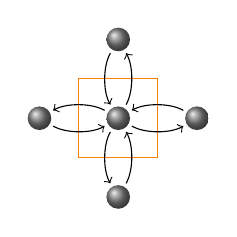
\begin{tikzpicture}[baseline, shorten >=2mm, shorten <=2mm]
    \foreach \point in {(0, 0), (-1, 0), (1, 0), (0, -1), (0, 1)} {
        \shade [ball color=gray] \point circle (1.5mm);
        }
    \draw [orange] (-0.5, -0.5) rectangle (0.5, 0.5);
    \foreach \point in {(-1, 0), (1, 0), (0, -1), (0, 1)} {
        \draw [<-] \point to [bend left]  (0, 0);
        \draw [->] \point to [bend right] (0, 0);
        }
\end{tikzpicture}

        \caption{unit cell}
        \label{square-lattice unit cell}
    \end{subfigure}%
    \begin{subfigure}[b]{4.666cm}
        \input{results/square_lattice/square_lattice_dispersion.sl}
        \caption{dispersion}
        \label{square-lattice dispersion}
    \end{subfigure}%
    \begin{subfigure}[b]{4.666cm}
        \input{results/square_lattice/square_lattice_dos.sl}
        \caption{density of states}
        \label{square-lattice dos}
    \end{subfigure}
    \caption[Square lattice]
        {Properties of the square tight-binding lattice.}
\end{figure}
%
In order to perform calculations beyond the approximation of a constant density
of states, some kind of model or experimental data which provides the necessary
electronic structure is required. Throughout the present work, a tight-binding
model of a square lattice will be applied for thus purpose. The unit cell with a
single basis atom is depicted in Fig.~\ref{square-lattice unit cell}, where
arrows represent the allowed electronic transitions. The defining
\name{Hamilton} operator in first quantization reads
%
\begin{equation*}
    \op H = -t \sum_{\vec R}
         [ \ket{\vec R + \vec t_1}
         + \ket{\vec R - \vec t_1}
         + \ket{\vec R + \vec t_2}
         + \ket{\vec R - \vec t_2} ]
    \bra{\vec R},
\end{equation*}
%
where the sum goes over all lattice sites $\vec R = n_1 \vec t_1 + n_2 \vec t_2$
with $n_1, n_2 \in \mathds Z$ at which the \name{Wannier} states $\ket{\vec R}$
are localized. $t$ is the nearest-neighbor coupling parameter, $\vec t_1 = [a \
0]$ and $\vec t_2 = [0 \ a]$ are the translation vectors of length $a$, the
lattice constant.

An expansion into \name{Bloch} states $\ket{\vec k}$ with $\vec k = [k_x \ k_y]$
via the \name{Fourier} transform
%
\begin{equation*}
    \ket{\vec R} = \int \D \vec k \, \E^{-\I \vec k \vec R} \ket{\vec k},
\end{equation*}
%
where the integration is e.g. over the first \name{Brillouin} zone, leads to the
dispersion relation
%
\begin{equation*}
    \epsilon(\vec k) = -2 t \, [\cos(k_x a) + \cos(k_y a)]
\end{equation*}
%
a contour plot of which is given in Fig.~\ref{square-lattice dispersion}.

Finally, the corresponding density of states per spin and unit cell, shown in
Fig.~\ref{square-lattice dos}, reads
%
\begin{equation*}
    n(\epsilon) = \frac{K \big(1 - (\tfrac \epsilon {4 t})^2 \big)}{2 \pi^2 t}
    \quad \text{where} \quad
    K(x) = \int \from 0 \till{\frac \pi 2} \D \varphi \,
    \big[ 1 - x \sin^2(\varphi) \big]^{-\frac 1 2}
\end{equation*}
%
is the complete elliptic integral of the first kind \cite[Eq.~4.146 and
4.147]{Czycholl08}. It features a \name{van Hove} singularity at the
\name{Fermi} level $\epsilon = 0$ at half-filling, at which is diverges
logarithmically \cite[Eq.~7]{Szczesniak06}. Since the density of states at the
chemical potential of the non-interacting system enters in the definition of the
coupling strengths in Eq.~\ref{coupling strengths}, which have to be finite,
well-defined quantities, a reduced particle number, namely quarter-filling, is
chosen in the following.

\section{Self-energy on real and imaginary axis}

\begin{figure}
    \small
    \input{results/self-energy/Delta(iomega).sl}
    \input{results/self-energy/Delta(omega).sl}
    \input{results/self-energy/chi(iomega).sl}
    \input{results/self-energy/chi(omega).sl}
    \input{results/self-energy/Z(iomega).sl}
    \input{results/self-energy/Z(omega).sl}
    \caption[Self-energy at different temperatures]{
        Imaginary- and real-axis self-energy components at different
        temperatures for a square-lattice density of states with an electronic
        bandwidth of $2 \, \unit{eV}$ at quarter-filling, a phonon frequency
        $\omega \sub E = 20 \, \unit{meV}$, an electron-phonon coupling strength
        $\lambda = 1$, a \name{Coulomb} pseudo-potential $\mu^* = 0.1$ and a
        cutoff frequency $\omega_N = 100 \, \omega \sub E$. Note that the
        displayed frequency ranges do not correspond to the cutoff.}
    \label{imaginary- and real-axis self-energy components}
\end{figure}
%
In Fig.~\ref{imaginary- and real-axis self-energy components} numerical
solutions of the local \name{Eliashberg} equations stated in Eqs.~\ref{local
Eliashberg equations} are shown together with the their \name{Padé} approximants
as presented in Section~\ref{Pade approximants}, analytically continued to the
real axis, for different temperatures. For all parameter sets used in this
work, the qualitative appearance of the resulting curves is the same:

On the imaginary-axis not only the renormalization $Z(\I \omega_n)$, in
accordance with Fig.~\ref{validation Pade}, but also the energy gap $\Delta(\I
\omega_n)$ and shift $\chi(\I \omega_n)$ are bell-shaped and centered at the
origin. The first-mentioned are always concave functions whereas the sign of
the latter may change, resulting in a convex curve as in the example.

Asymptotically, the energy gap approaches the negative or vanishing constant
\name{Coulomb} contribution given in Eq.~\ref{constant Coulomb contribution},
the renormalization goes to unity and the energy shift vanishes, but much more
slowly than the former two.

The maybe most characteristic property of the energy gap is its temperature
dependence, further discussed in the subsequent section, through which it is
qualified as an order parameter for the superconducting state. With rising
temperature it decreases with increasing speed towards zero, which is reached,
by definition, at the critical temperature. In principal, this process affects
the magnitude rather than the shape of the curve, resulting in a common zero of
the displayed family of curves or, more precisely, of their analytic
continuations, since naturally the solution is discrete on the imaginary axis
and does not include this very point in general. Over the same temperature
range, the other two quantities barely change.

On the real axis the shapes turn out to be more complicated. The renormalization
$Z(\omega)$ basically resembles the analytic one, shown in Fig.~\ref{validation
Pade}, the properties of which have already been discussed. One of them, namely
the vanishing imaginary part at frequencies below the renormalized phonon
frequency, is recognized in the energy gap $\Delta(\omega)$ and shift
$\chi(\omega)$ as well. The former even features the aforementioned peaks, in
the vincinity of which the exact behavior of the \name{Padé} approximants is
untrustworthy for being very sensitive to parameter changes. Beyond the peak,
the real and imaginary parts of the energy gap describe arches of opposite
orientation. The asymptotes of all quantities are the same as on the
imaginary-axis, although in the case of the energy shift this does not become
apparent from the depicted detail.

\subsection{Temperature dependence of order parameter}
\label{temperature dependence of order parameter}

\begin{figure}
    \small
    \centering
    \input{results/order_parameter/order_parameter.sl}
    \caption[\name{Eliashberg} gap]{
        Order parameters. The temperature dependence of leading \name{Matsubara}
        and measurable gap is shown for the same parameter set as in
        Fig.~\ref{imaginary- and real-axis self-energy components}, except for a
        lower cutoff frequency $\omega_N = 15 \, \omega \sub E$. The phase
        transition in characterized by a diverging number of iterations needed
        to reach self-consistency.}
    \label{order parameter}
\end{figure}
%
Leaving the invariant shape of the energy gap on the imaginary frequency axis
out of account, the temperature dependence of its magnitude, represented by its
value at the first \name{Matsubara} frequency, is shown in Fig.~\ref{order
parameter}, supplemented by the corresponding curve for the energy gap which is
actually measurable in experiments and defined by the fixed-point equation
\cite[Eq.~3a]{VidbergSerene77}
%
\begin{equation} \label{measurable gap}
    \Delta_0 = \Re[\Delta(\Delta_0)].
\end{equation}
%
Both curves turn out to be very similar: Starting at absolute zero, they remain
nearly constant at first and subsequently become ever steeper approaching the
critical temperature at which they vanish. They resemble the well-known BCS
result, exemplified in Fig.~\ref{BCS gap}, which changes exponentially and like
a square root near $T = 0$ and $T \sub c$, respectively
\cite[Eq.~11.60]{Czycholl08}.

Fig.~\ref{order parameter} also shows how the number of iterations needed to
obtain a self-consistent solution of the \name{Eliashberg} equations increases
drastically at the critical temperature. This is due to the magnitude of the
energy gap converging much slower than its shape \cite[185]{VidbergSerene77}.
Enforcing the normal-state property $\Delta = 0$ yields similar convergence
rates at all temperatures, $T \sub c$ included.

\section{Convergence tests}

It is now investigated how the results are influenced by the choices of, first,
the cutoff frequency of the \name{Matsubara} sums and, secondly, the number of
points used for the quadrature of the energy integrals, which are both mandatory
for a computational implementation of the \name{Eliashberg} equations. This
knowledge is necessary to obtain confidence in all subsequent results.

\subsection{Convergence of self-energy with cutoff frequency}

\begin{figure}
    \small
    \begin{minipage}{4.666cm}
        \input{results/cutoff/Delta_N(iomega).sl}
    \end{minipage}%
    \begin{minipage}{4.666cm}
        \input{results/cutoff/chi_N(iomega).sl}
    \end{minipage}%
    \begin{minipage}{4.666cm}
        \input{results/cutoff/Z_N(iomega).sl}
    \end{minipage}%
    \caption[Cutoff-induced errors of self-energy]{
        Comparison to expose cutoff-induced errors in the components of the
        self-energy. Except for the cutoff and a temperature $T = 1 \, \unit K$,
        the settings are as for the results displayed in Figs.~\ref{imaginary-
        and real-axis self-energy components} and \ref{order parameter}.}
    \label{cutoff dependence of the self-energy}
\end{figure}
%
In Fig.~\ref{cutoff dependence of the self-energy} the self-energy components
on the imaginary axis are shown for different cutoff frequencies. Since a low
temperature has been chosen, the \name{Matsubara} frequencies lie sufficiently
close together to use line rather than scatter plots.

It turns out that the sensitivities of different quantities to the cutoff
frequency differ. The energy shift proves to be affected most, especially near
the cutoff itself where it decays spontaneously. A similar behavior, but much
less pronounced, is found for the renormalization, in contrast to the energy gap
which exhibits the correct asymptotes. Regarding the magnitude it becomes
evident that the energy gap is favored by a low cutoff whereas renormalization
and energy shift are suppressed.

With the above results in mind one could argue that an application of the
imaginary-axis \name{Eliashberg} equations at low frequencies, where the
computational workload is small, is pointless, at least being interested in more
than qualitative tendencies. Nevertheless, when determining the critical
temperature, the artifacts of the cutoff in the frequency dependence of the
self-energy will be of minor importance.

\subsection{Convergence of \bm$T \sub c$ with cutoff frequency}

\begin{figure}
    \small
    \begin{subfigure}{7cm}
        \input{results/convergence/cutoff_frequency.sl}
        \caption{square lattice at quarter-filling}
    \end{subfigure}%
    \begin{subfigure}{7cm}
        \input{results/convergence/cutoff_frequency_cdos.sl}
        \caption{constant density of states}
    \end{subfigure}
    \caption[Convergence with cutoff frequency]{
        Convergence with cutoff for a phonon frequency $\omega \sub E = 20 \,
        \unit{meV}$, an electron-phonon coupling strength $\lambda = 1$ and a
        \name{Coulomb} pseudo-potential $\mu^* = 0.1$. In each panel, the latter
        is rescaled differently.}
    \label{convergence with cutoff frequency}
\end{figure}
%
The quantity to be handled with most care regarding the cutoff is the
\name{Coulomb} pseudo-potential already discussed in Section~\ref{introduction
of cutoff frequency}, which led to the introduction of a rescaled quantity. In
order to point out the benefits of the latter, in Fig.~\ref{convergence with
cutoff frequency} the critical temperature is shown as a function of the cutoff
frequency for both a constant and a rescaled \name{Coulomb} pseudo-potential.

Depending on whether the density of states is assumed to be constant or not,
different rescaling prescriptions have to be used. For the CDOS approximation,
Eq.~\ref{CDOS rescaled Coulomb pseudo-potential} can be directly applied.
Otherwise one has to resort to Eq.~\ref{rescaled Coulomb pseudo-potential} which
unfortunately involves the original coupling constant $\mu \sub C$ rather than
\name{McMillan}'s \name{Coulomb} pseudo-potential $\mu^*$. Hence, in order to
obtain roughly comparable results in both cases, whenever the density of states
is taken into account the first step is to estimate $\mu \sub C$ from $\mu^*$
which is done via Eq.~\ref{McMillan's Coulomb pseudo-potential}, where $E \sub
B$ is assumed to be half the electronic bandwidth.

It is confirmed that within the CDOS approximation the rescaling is required in
order to yield convergent results. This does not apply to the \name{Eliashberg}
equations in general since within nothing but the local approximation one has
convergence in any case; it is just considerably faster if an appropriate
rescaling is performed. The CDOS convergence rate is not reached though.

An enhancement of the critical temperature with increasing cutoff frequency for
a constant \name{Coulomb} pseudo-potential is in accordance with the fact that
an appropriately rescaled \name{Coulomb} pseudo-potential behaves similarly,
since the \name{Coulomb} interaction opposes superconductivity
\cite[1038]{Carbotte90}. Having performed the rescaling, one is left with a
decreasing curve which may be ascribed to results for the order parameter
presented in Fig.~\ref{cutoff dependence of the self-energy}.

Until now is has been taken for granted that the cutoff is defined in terms of
frequency rather than a specific number of \name{Matsubara} frequencies. The
latter is thus defined by the cutoff frequency and the temperature together.
Hence, in Fig.~\ref{convergence with cutoff frequency} it varies both along the
horizontal and the vertical axis. The reason for this definition of the cutoff
is that, as stated above, the shape of the self-energy as a function of
frequency does not change much with temperature.

\subsection{Convergence of \bm$T \sub c$ with energy resolution}

\begin{figure}
    \small
    \centering
    \input{results/convergence/integration_points.sl}
    \caption[Convergence with number of integration points]{
        Convergence with the number of integration points for two different
        phonon frequencies. Constants are defined as in Fig.~\ref{order
        parameter}.}
    \label{convergence with energy resolution}
\end{figure}
%
The remaining quantity by which the accuracy of numerical solutions is limited,
is the number of points used for discretizing the integrands in Eqs.~\ref{local
Eliashberg equations}. The quadrature is performed using the trapezoidal rule
and the energy points chosen equally spaced.

As can be seen in Fig.~\ref{convergence with energy resolution}, the occurring
errors are not as predictable as in Fig.~\ref{convergence with cutoff
frequency}, where the critical temperature was shown to converge with the cutoff
frequency following continuous curves. Instead, the resulting critical
temperatures are scattered apparently at random (of cause each calculation alone
is deterministic) around the correct value, loosely bounded by radii with shrink
with increasing resolution.

As already anticipated in the caption of Fig.~\ref{CDOS at low frequencies}, the
errors are larger for lower phonon frequencies, which correspond to lower
temperatures at which the \name{Lorentz} functions to be integrated over are
sharper and thus only resolved accurately if neighboring sample points are very
close. Theoretically, it is also possible to guarantee the same precision for
all temperatures with a constant number of points. But this requires an
intelligent, non-equidistant sampling.

\section{\name{McMillan}'s equation for \name{Einstein} spectra}

\begin{table}
    \centering
    \input{results/mcmillan/mcmillan.dat}
    \caption{
        $T \sub c \pm 0.001 \, \unit K$ for different $\lambda$ and $\mu^*$ with
        $\omega \sub E = 20 \, \unit{meV}$.}
    \label{Tc table}
\end{table}
%
\begin{figure}
    \small
    \begin{subfigure}{7cm}
        \input{results/mcmillan/mcmillan_1st.sl}
        \caption{$\mu^* = 0$}
    \end{subfigure}%
    \begin{subfigure}{7cm}
        \input{results/mcmillan/mcmillan_2nd.sl}
        \caption{$\mu^* > 0$}
    \end{subfigure}
    \caption[\name{McMillan}'s fits]{
        Combined representation of \name{McMillan}'s original data and lines of
        best fit together with their newly calculated counterparts for an
        \name{Einstein} phonon spectrum.}
    \label{McMillan's fits}
\end{figure}
%
Having shown that the numerical results are stable and satisfy the qualitative
expectations, the next step is a direct comparison with a well-established
result, namely \name{McMillan}'s equation for the critical temperature. It was
derived starting from the CDOS \name{Eliashberg} theory, so that the latter
should reproduce the results of the former at least approximately.

If there is any justifiable discrepancy between the original and the present
work it is due to the electron-phonon spectral function or, more precisely, the
phonon density of states. Whereas \name{McMillan} performed his calculations for
niobium, now a simple \name{Einstein} spectrum is assumed. Interestingly, in
place of the peak at the \name{Einstein} frequency in the real-axis self-energy
displayed in Fig.~\ref{imaginary- and real-axis self-energy components}, the
analogous result of \name{McMillan} \cite[Fig.~4]{McMillan68} features two peaks
which also appear in the phonon density of states of niobium.

Back on topic, the aim of this section is to derive an alternative $T \sub c$
formula which differs from \name{McMillan}'s only by the three fit parameters
which are adjusted to an \name{Einstein} spectrum, i.e. a single phonon
frequency, $\omega \sub E = 20 \, \unit{meV}$ in this case.

To that end, the first step is to determine critical temperatures for different
electron-phonon coupling strengths and \name{Coulomb} pseudo-potentials.
(\name{McMillan} calculated $\lambda$ for different $T \sub c$ and $\mu^*$.) The
results are listed in Table~\ref{Tc table}. The second step is to perform the
linear regressions for Eqs.~\ref{linear regression formulas} applying the usual
least-squares method. This is visualized in Fig.~\ref{McMillan's fits}. The fit
parameters turn out to be $A = 0.94 \pm 0.03$, $B = 1.11 \pm 0.01$ and $C = 0.74
\pm 0.01$. Hence,
%
\begin{equation*}
    T \sub c \super E = \frac{\omega \sub E}{0.94} \exp \bigg[ {-\frac
        {1.11 \, (1 + \lambda)}
        {\lambda - 0.74 \lambda \mu^* - \mu^*}}
    \bigg].
\end{equation*}

\section{Critical-temperature benchmarks}

\begin{figure}
    \small
    \input{results/benchmark/tc_lamda.sl}
    \input{results/benchmark/tc_lamda_2.sl}
    \input{results/benchmark/tc_omegaE.sl}
    \input{results/benchmark/tc_muStar.sl}
    \caption[Critical-temperature benchmarks]{
        Comparison of the critical temperatures according to \name{McMillan}'s
        formula in its original form and with its constants adjusted to an
        \name{Einstein} phonon spectrum as well as the local \name{Eliashberg}
        equations, either within the approximation of a constant density of
        states or for a square lattice with an electronic bandwidth of $2 \,
        \unit{eV}$ at quarter-filling. As constants, an \name{Einstein}
        frequency $\omega \sub E = 20 \, \unit{meV}$, an electron-phonon
        coupling $\lambda = 1$ and a \name{Coulomb} pseudo-potential $\mu^* =
        0.15$ are chosen. The \name{Matsubara} sum is cut off at $\omega_N = 15
        \, \omega \sub E$. 2001 points were used for the numerical solution of
        the energy integral.}
    \label{critical-temperature benchmarks}
\end{figure}
%
At this point a comparison of local and CDOS \name{Eliashberg} theory as well as
\name{McMillan}'s formula, both original and adjusted, can be performed.
Therefor, $T \sub c$ is calculated for different $\omega \sub E$, $\lambda$ and
$\mu^*$ whereby only one parameter is varied at a time and the others are held
constant. The results are presented in Fig.~\ref{critical-temperature
benchmarks}.

Altogether, a very good agreement can be reported. As expected, the adjusted
version of \name{McMillan}'s formula does best in reproducing the critical
temperature according to CDOS \name{Eliashberg} theory for \name{Einstein}
spectra. The original formula works comparably good but it slightly
underestimates the dependence on the \name{Coulomb} pseudo-potential and already
fails at lower electron-phonon coupling strengths. However, it is well known
that \name{McMillan}'s formula intrinsically underestimates $T \sub c$ for large
$\lambda$ \cite{AllenDynes75}. It predicts the upper bound
%
\begin{equation*}
    \lim_{\lambda \rightarrow \infty} T \sub c = \frac {\av \omega} A
    \exp \bigg[ -\frac B {1 - C \mu^*} \bigg],
\end{equation*}
%
whereas \name{Eliashberg} theory states an asymptotic behavior proportional to
$\sqrt \lambda$ \cite[Eq.~3.56]{Galasso05}.

The differences between the results of the \name{Eliashberg} theory for constant
and square-lattice densities of states are acceptable, especially if the
heuristic mapping from $\mu^*$ to $\mu \sub C$ is taken into account. There is
no general solution to resolve this ambiguity. Nevertheless, it still remains
unclear to what extend the critical temperature is determined by the shape of
the density of states in the vicinity of the chemical potential, since the
square lattice at quarter filling, which has only been analyzed so far, is
rather benign in this regard. This question is further investigated in the
following section.

Apart from the comparison of the different theories,
Fig.~\ref{critical-temperature benchmarks} gives a good overview of the general
dependence of the critical temperature on the characteristic variables. Large
values of $\lambda$ and $\omega \sub E$ favor superconductivity, while $\mu^*$
opposes it. Concerning $\omega \sub E$, the proportionality which is immanent in
\name{McMillan}'s formula is perfectly confirmed. It is responsible for the
isotope effect and may be explained by the fact that $\omega \sub E$ enters the
\name{Eliashberg} equations only through $\lambda(n)$ or the phononic
\name{Green} function, the \q{broadening} of which is determined by $\frac T
{\omega \sub E}$.

\section{Energy dependence}

\begin{figure}
    \small
    \centering
    \input{results/energy/energy_dos.sl}
    \input{results/energy/energy_shift.sl}
    \input{results/energy/energy_tc.sl}
    \caption[Energy dependence]{
        Energy dependence. It is shown how the critical temperature, the
        self-consistent chemical potential and the leading energy shift change
        with the chemical potential of the non-interacting system. Again, the
        parameters are the same as in Fig.~\ref{order parameter}.}
    \label{energy dependence}
\end{figure}
%
The final survey regarding the single-band \name{Eliashberg} theory is concerned
with the dependence of the critical temperature on the shape of the density of
states near the chemical potential, where the superconducting pairing takes
place.

This is done by \q{scanning} the entire domain of the density of states of the
square lattice by varying the chemical potential of the non-interacting system
with respect to which the coupling strengths are defined. In addition to the
critical temperature the change in the chemical potential (in order to conserve
the particle number) and the leading value of the energy shift are determined.
The results are shown in Fig.~\ref{energy dependence} together with a plot of
the density of states. Note that the magnitude of the density of states only
enters through the coupling strengths which are held constant.

The following interpretation is guided by the observations that a high density
of states is generally favorable for superconductivity and that not only its
value at one exact energy contributes, but rather floating averages with respect
to bell-shaped weight functions which are centered at $\mu - \chi(\I \omega_n)$,
which can be directly deduced from Eq.~\ref{local Eliashberg equations}.

Although $\chi(\I \omega_n)$ is partially compensated by the change of the
chemical potential $\mu_0 - \mu$ \cite[80]{AllenMitrovic82}, as can be seen in
the central panel of Fig.~\ref{energy dependence}, it still determines the
direction of the effective energy shift. More precisely, only for small
\name{Matsubara} frequencies $\chi(\I \omega_n)$ exceeds the constant $\mu_0 -
\mu$ in magnitude, but these are the ones with the dominant contribution. Hence,
the focus is on $\chi(\I \omega_n)$, which always shifts the center of the
floating average towards a higher density of states.

Very close to the \name{van Hove} singularity and the band edges the critical
temperature is lower than expected because the density of states entering the
coupling constant does not represent the average density of states in the
vicinity, which is less. At the singularity itself the electron-phonon matrix
element and, for example, the \name{Hubbard} parameter must vanish in order to
justify the definition of finite coupling constants. If a critical temperature
shall be ascribed to this case at all, it must be zero.

In between these extremes the situation is different: Approaching the \name{van
Hove} singularity from one of the sides, the center of the floating average is
continuously shifted towards more favorable energies, albeit with decreasing
magnitude, hence the slow decrease of the critical temperature. However, in the
proximity of the \name{van Hove} singularity the steep slope of the density of
states overcompensates this effect, which leads to a boost of the critical
temperature shortly before it drops towards zero.

To conclude, the shape of the density of states may affect the critical
temperature considerably, especially where changes with energy are strong, e.g.
at \name{van Hove} singularities. This is a problem inherent in the definition
of the coupling strengths, which should give a reliable measure of the real
coupling. A possible solution is to use intensive coupling strengths which are
defined with respect to wave functions rather than the density of states
\cite{PickettKlein81}.
